% !TeX document-id = {78aa9ab2-f337-4819-975a-aa2344baa597}
%
% Niniejszy plik stanowi przykład formatowania pracy magisterskiej na
% Wydziale MIM UW.  Szkielet użytych poleceń można wykorzystywać do
% woli, np. formatujac wlasna prace.
%
% Zawartosc merytoryczna stanowi oryginalnosiagniecie
% naukowosciowe Marcina Wolinskiego.  Wszelkie prawa zastrzeżone.
%
% Copyright (c) 2001 by Marcin Woliński <M.Wolinski@gust.org.pl>
% Poprawki spowodowane zmianami przepisów - Marcin Szczuka, 1.10.2004
% Poprawki spowodowane zmianami przepisow i ujednolicenie 
% - Seweryn Karłowicz, 05.05.2006
% Dodanie wielu autorów i tłumaczenia na angielski - Kuba Pochrybniak, 29.11.2016

% dodaj opcję [licencjacka] dla pracy licencjackiej
% dodaj opcję [en] dla wersji angielskiej (mogą być obie: [licencjacka,en])




\documentclass[en]{pracamgr}

%\usepackage{dingbat}

\usepackage{amsmath}
\usepackage{amsfonts} 


%% Imports the package natbib
\usepackage[square,numbers]{natbib}
\usepackage{xcolor}
\usepackage{graphicx}
\usepackage{hyperref}



%% Sets the bibliography style
\bibliographystyle{abbrvnat}

% Dane magistranta:
\autor{Marta Nowakowska}{385914}

% Dane magistrantów:
%\autor{Autor Zerowy}{342007}
%\autori{Autor Pierwszy}{342013}
%\autorii{Drugi Autor-Z-Rzędu}{231023}
%\autoriii{Trzeci z Autorów}{777321}
%\autoriv{Autor nr Cztery}{432145}
%\autorv{Autor nr Pięć}{342011}

\title{Time series prediction using self-attention models}
\titlepl{Prognozowanie szeregów czasowych przy użyciu modeli z uwagą}

%\tytulang{An implementation of a difference blabalizer based on the theory of $\sigma$ -- $\rho$ phetors}

%kierunek: 
% - matematyka, informacyka, ...
% - Mathematics, Computer Science, ...
\kierunek{Computer Science}

% informatyka - nie okreslamy zakresu (opcja zakomentowana)
% matematyka - zakres moze pozostac nieokreslony,
% a jesli ma byc okreslony dla pracy mgr,
% to przyjmuje jedna z wartosci:
% {metod matematycznych w finansach}
% {metod matematycznych w ubezpieczeniach}
% {matematyki stosowanej}
% {nauczania matematyki}
% Dla pracy licencjackiej mamy natomiast
% mozliwosc wpisania takiej wartosci zakresu:
% {Jednoczesnych Studiow Ekonomiczno--Matematycznych}

% \zakres{Tu wpisac, jesli trzeba, jedna z opcji podanych wyzej}

% Praca wykonana pod kierunkiem:
% (podać tytuł/stopień imię i nazwisko opiekuna
% Instytut
% ew. Wydział ew. Uczelnia (jeżeli nie MIM UW))
\copiekun{dr hab. Piotr Miłoś\\
	Institute of Mathematics, Polish Academy of Sciences\\
}

\opiekun{dr hab. Marek Cygan, prof. UW\\
	University of Warsaw\\
}

%\coopiekun{dr Piotr Miłoś\\
%	Institute of Mathematics, Polish Academy of Sciences\\
%}

% miesiąc i~rok:
\date{September 2022}

%Podać dziedzinę wg klasyfikacji Socrates-Erasmus:
\dziedzina{ 
	%11.0 Matematyka, Informatyka:\\ 
	%11.1 Matematyka\\ 
	%11.2 Statystyka\\ 
	11.3 Informatics, Computer Science\\ 
	%11.4 Sztuczna inteligencja\\ 
	%11.5 Nauki aktuarialne\\
	%11.9 Inne nauki matematyczne i informatyczne
}

%Klasyfikacja tematyczna wedlug AMS (matematyka) lub ACM (informatyka)
\klasyfikacja{I. Computing Methodologies\\
	I.2. Artificial Intelligence\\
	I.2.6. Learning \\
	Connectionism and neural nets}

% Słowa kluczowe:
\keywords{Time series, Neural network, Transformer, Self-attention model}

% Tu jest dobre miejsce na Twoje własne makra i~środowiska:
\newtheorem{defi}{Definition}[section]
\newcommand{\pk}[1]{\textcolor{red}{\small [pk: #1]}}
\newcommand{\mn}[1]{\textcolor{purple}{\small [mn: #1]}}


% koniec definicji

\begin{document}
	\maketitle
	
	\begin{abstract}
		The Transformer model has excelled at various sequence-processing problems. However, the past works dedicated to time series forecasting with neural networks commonly simplified this task to predicting parameters of simple distributions, i.e. the Gaussian distribution. This thesis explores the idea of applying the Transformer to forecasting parameters of a granular categorical distribution for each predicted data point. This model is compared against the Gaussian distribution-based Transformer in the presented experiments.
		
	\end{abstract}
	
	\tableofcontents
	%\listoffigures
	%\listoftables
	
	\chapter*{Introduction}
	\addcontentsline{toc}{chapter}{Introduction}
	
	\section*{Time series and their importance}\label{r:tsi}
	
	Forecasting future values and their probability distribution on the basis of historical data points is one of the most prevalent problems in both industry and research.
	For example, time series analysis can be used for predicting the number of ride-hailing trips completed during special events like holidays (\cite{uber}), but also for estimating stock market behavior (\cite{stock1}) and solving resource allocation tasks (\cite{graph-forecast}). 
	
	
	This wide usage brought time series a lot of attention in the past. Some of the most known methods for their forecasting are based on the Box-Jenkins method like the ARIMA (autoregressive integrated moving average) \cite{arima} model, but there also exist ones using the exponential smoothing techniques and state space models \cite{ssm}. Despite their popularity, they come with some fundamental disadvantages. For example, they need to be fitted separately for every similar sequence (\cite{enhancing}, \cite{deepar}) and cannot be trained to recognize these similarities which makes using them time-inefficient in the long term.
	Furthermore, these models typically use parameters that have to be handpicked by the user (\cite{enhancing},
	\cite{deepar}), which makes them more suitable for field experts with knowledge of both parameter selection procedure and preferably time series' behavior.
	
	
	The aforementioned issues are not a problem for deep neural networks, since they can be trained to recognize a group of similar time series and their hyper-parameters have to be only selected once for the training and not at the prediction time. What is more, once trained neural networks can be adapted to new data using transfer learning. 
	
	On top of that, neural networks proved to be very successful in other fields, including natural language translation, which is a problem with similar properties to time series forecasting. In particular, the translation can be defined as a mapping of one sequence to a second one, similarly to how one can map historical values to future ones. Thus, the achievements of the natural language processing (NLP) field, including RNN models have almost directly transferred to time series forecasting. However, RNNs and their successors (LSTM \cite{lstm}, GRU \cite{gru}) have difficulty with long sequences \cite{context}, causing them to struggle with time series that can contain long-term dependencies.
	
	The next important step in the development of deep neural network adaptations for time series forecasting was the Transformer \cite{tr}. Instead of using recurrent networks, it relies almost entirely on the self-attention mechanism, which can be trained to estimate dependencies in arbitrarily long sequences, making it possible for the model to deal with larger-scale forecasting.
	However, there are problems with integrating it directly for time series forecasting usage. One of them is that the scaled dot-product attention can only capture dependencies between particular data points, but it cannot fully use the time series' local shape, which makes it struggle with capturing its seasonality and other patterns or anomalies (\cite{enhancing}).
	One solution to that problem was proposed in \cite{enhancing} by introducing convolutional self-attention.
	
	
	
	\section*{Problem statement}\label{r:problemst}
	
	Previously neural networks including the Transformer were commonly used for predicting parameters of a simple distribution like Gaussian per each forecasted point in time (\cite{deepar}, \cite{enhancing}). This work expands that idea to modeling any continuous distribution by approximating it with a categorical one. We present a comparison of both methods on commonly used datasets and metrics.
	
	
	\section*{Contributions}\label{r:contributions}
	
	The work described in this thesis has been done via a collaboration with scientists from the Institute of Mathematics of the Polish Academy of Sciences.
	
	My most important contributions are:
	\begin{enumerate}
		\item Gaussian distribution-based Transformer
		\item Experiments with the Gaussian distribution-based Transformer
		\item Base implementation of the dataset feeder
		\item Time features as in \cite{enhancing} (on the data feeding side)
	\end{enumerate}
	
	\chapter{Background}\label{r:background}
	
	\section{Time series and notation}
	
	We define time series as a sequence of real numbers measured across time with a constant \textbf{frequency}. Frequency is defined in time units, e.g. weeks, days, or hours. For multiple time series represented as a matrix $\textbf{y}$, where each row is a separate time series, $y^{(i)}_t$ denotes $t$ time step of a series number $i$.
	
	One can extend the definition above to a sequence of any data type, but it is not necessary for the datasets that we use for this thesis.
	
	
	\section{Transformer model architecture}\label{s:architecture}
	
	Transformer \cite{tr} is a deep neural network model that relies on a scaled dot-product attention mechanism introduced in the same paper. There exist some modifications to the model presented in \cite{tr}, but we follow the "decoder-only" \cite{wikipedia} architecture type.
	
	\subsection{Overview}
	
	\begin{figure}[ht!]
		\centering
		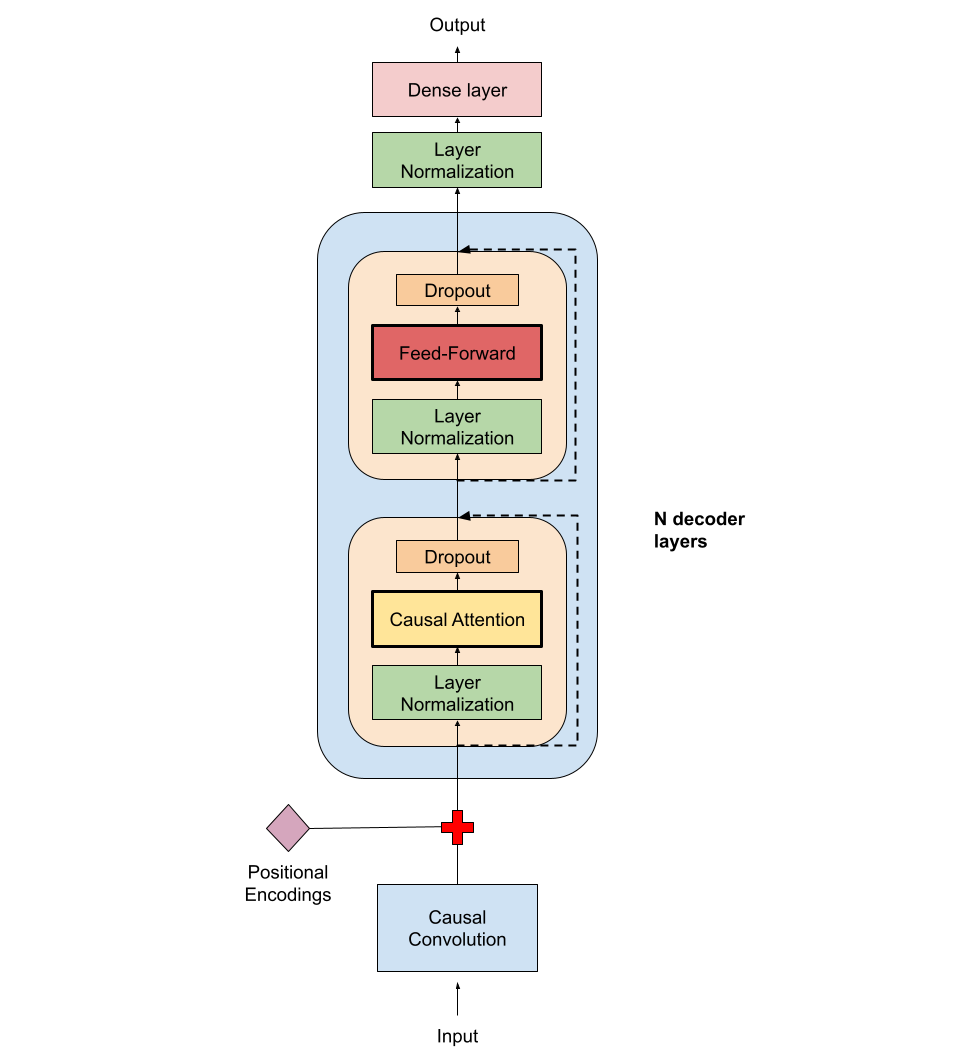
\includegraphics[height=130mm]{decoder3.png}
		\caption{Transformer's architecture. The dotted lines represent residual connections. \label{our-decoder}}
	\end{figure}
	
	
	
	Our implementation of the Transformer model consists mainly of a causal convolution layer, positional encoding layer, $N$ identical decoder layers, layer normalization, and a fully-connected layer. 
	Most of the layers' outputs have $d_{model}$ dimension.
	I present the general architecture in Figure ~\ref{our-decoder}.
	
	\textbf{Positional encoding} allows us to feed the model embedded information about how the data points are ordered in the inputted time series.
	We use a trainable embedding for the positional encoding and add it to the input before it reaches the first decoder layer.
	
	A single \textbf{decoder} layer consists of a causal attention sub-layer and a feed-forward sub-layer:
	\begin{itemize}
		\item The feed-forward sub-layer contains a simple feed-forward neural network with two dense layers and a ReLU activation in-between.
		\item The causal attention sub-layer contains the attention mechanism that I describe later on.
	\end{itemize}
	
	Both sub-layers are residual and wrapped with a layer normalization and a dropout layer.
	
	\section{Attention}
	
	\subsection{Scaled Dot-Product Attention}
	
	Attention is the key to explaining how the Transformer works.
	It enables us to train the neural network to encode the relations between different parts of the input (e.g., a time series' data points).
	
	Scaled dot-product attention introduced along with the Transformer architecture in \cite{tr} is perhaps the most known kind of attention function.
	One can informally see its calculation as operations on a neural network-approximated dictionary with vector keys and corresponding values. We use a dot operation between the query being matched and the dictionary's keys as a measure of similarity. When they are orthogonal, the dot product will be equal to 0. On the other hand, for vectors of fixed length, the dot product is maximal when they have the same direction.
	
	To calculate the attention score vector between one data point and every that comes after, one first needs to provide a query vector for the first data point and a set of vector pairs consisting of keys and values for all the other data points. We match our query against all of the keys by a dot product and use the softmax function to normalize the result. When the result of softmax is large between two data points, we can informally say that the attention relates them. 
	Finally, by multiplying the softmax results with the corresponding values we get a set of weighted values vectors. After summing them we get the attention score vector for one data point.
	\newline
	
	In reality, we do not need to calculate the attention sequentially for every data point, but rather use matrix operations.
	One needs to provide three matrices to the attention layer: $Q, K \in \mathbb{R}^{d_I \times d_k}, V \in \mathbb{R}^{d_I \times d_v}$ (respectively called queries, keys and values). They are created by multiplying the input matrix $I \in \mathbb{R}^{d_I \times d_{model}}$ with three distinct trainable weight matrices $W_Q \in \mathbb{R}^{d_{model} \times d_k}, W_K \in \mathbb{R}^{d_{model} \times d_k}, W_V \in \mathbb{R}^{d_{model} \times d_v}$.
	
	For given $Q, K, V$ we compute the attention with the following formula:
	
	$$ Attention(Q, K, V) = softmax(\frac{QK^{T}}{\sqrt{d_k}} - M)V \textrm{ (from \cite{enhancing})} $$
	
	where $d_k$ stands for the dimension of $Q$ and $K$. Dividing by its square root is supposed to balance out the growth of $Q$ and $K^{T}$ dot product that occurs with larger values of $d_k$.
	
	$M$ is a \textbf{mask matrix} that sets all the elements corresponding to connections between future and past (upper triangular) to $-\infty$. It prevents the model from attempting to relate past events to future ones.
	
	While calculating the softmax score for any two data points in a time series, the scaled dot-product attention does not use any information about other data points. We call this property \textbf{context-blindness}. Sometimes this might lead the model to assign a strong attention score between events that have similar values, even if their contexts (neighboring data points) are very different. That might cause the model to incorrectly recognize patterns in the time series (\cite{enhancing}). %\pk{\leftthumbsup}
	
	\subsection{Convolutional Attention}
	
	\textbf{Causal convolution} is a convolution used on input padded with $k - 1$ zeros at the start, where $k$ denotes the size of the kernel.
	
	%
	This type of convolution is particularly useful for time series since it enables us to make predictions with only partial input, essentially generating a completely new time series.
	\newline
	
	The convolutional attention \cite{enhancing} is calculated in almost the same way as the scaled dot-product attention. 
	It only differs in the way it computes queries and keys.
	Instead of applying a matrix multiplication with weight matrices, it uses a causal convolution with a stride of 1. When the kernel's size is equal to 1 it is equal to the matrix multiplication.
	
	The usage of convolution is supposed to offset the dot-product attention's context blindness. Since the convolution layer learns to recognize the input's context, a stronger attention score should be assigned to similar events.
	
	\subsection{Multi-headed attention}
	
	Each attention block might contain more than one parallel attention layer, aka the attention "head". In theory, this allows for different layers to learn various kinds of relationships in the input and is a very successful tool e.g. in natural language processing \cite{tr}.
	
	The outputs of all $h$ attention heads are concatenated and multiplied by a weight matrix $W^O \in \mathbb{R}^{hd_{v} \times d_{model}}$ to squeeze them back into $d_I \times d_{model}$ shape before passing them to the next layer.
	
	To offset the additional computational cost related with multiple attention heads, we set $d_k$ and $d_v$ to $d_{model} / h$.
	
	\section{Training}
	
	\subsection{Additional input}
	
	Following \cite{enhancing}, we use additional variables as part of the model's input aside from the time series itself.
	There are three kinds of additional input we use:
	\begin{enumerate}
		\item Numerical information about the time the input was recorded (year, month, day-of-the-week, hour-of-the-day, minute-of-the-hour). 
		
		\item Identifier of the time series.
		
		\item Input's distance from the sequence's start. 
		
	\end{enumerate}
	We embed all of the additional variables to the same dimension, sum those embeddings and normalize them. Finally, we add the result to our model's (embedded) input and normalize it as well.
	
	
	\subsection{Scaling and weighted sampling}\label{s:scale}
	
	The time series in a single dataset can vary in their ranges, which might obstruct the model's learning process. Due to the network's non-linearities, it needs to size down the input in its first layer and then reverse this scaling on the output (\cite{deepar}). Therefore, following \cite{enhancing} and \cite{deepar} we scale the input and output by respectively dividing and multiplying them by a scale factor $v_i$:
	
	$$ v_i = r + \frac{\sum^{T}_{t=1} y^{(i)}_t}{T} \text{,}$$
	where $T$ is $y^{(i)}$'s length and $r$ is a regularization term.
	
	Furthermore, we adopt a weighted sampling technique in our training, similarly to \cite{enhancing} and \cite{deepar}. Its main purpose is to counteract the model's tendency to underfit large-scale data since it occurs more rarely in the datasets. 
	We calculate the weights by normalizing the scale factor $v_i$.
	
	\section{Metrics}
	
	\subsection{Quantile loss}
	
	Quantile loss is a metric designed to evaluate and/or train models designed with quantile prediction in mind.
	We define $\rho$-quantile loss as follows:
	
	$$ QL_\rho(\hat{y}, y) = max(\rho(y - \hat{y}), (\rho - 1)(y - \hat{y})) \text{,} $$
	
	where $\hat{y}$ denotes the model's prediction for the $\rho$ quantile and $y$ is the ground truth value.
	
	This metric is characterized by a stronger penalization of over-predictions for $\rho$ smaller than 0.5, and under-predictions for $\rho$ greater than 0.5.
	
	\subsection{Risk metric}\label{s:risk}
	
	$Risk_\rho$ is a type of normalized quantile loss metric defined as follows for $\rho \in (0,1)$:
	
	$$ Risk_\rho(\hat{\textbf{y}}, \textbf{y}) 
	= 2\frac{\sum_{i,t}QL_\rho(\hat{y}^{(i)}_t, y^{(i)}_t)}
	{\sum_{i,t} |y^{(i)}_t|}$$
	
	It is very popular in time series prediction papers that use the Transformer (e.g. in \cite{enhancing}, \cite{deepar}), which leads us to choose it as the metric we use in the model's evaluation. Furthermore, quantile loss allows us to assess how well our model estimates the series' extreme values. It is useful for applications like electricity consumption risk estimation, where one might ask how likely it is in the given time frame that the power consumption reaches a certain level.
	
	\chapter{Approximating a continuous distribution with the Transformer}
	
	While the Transformer has already proven to be a very efficient tool for time series prediction, we believe it has a lot more potential that could be used without changing its architecture. In the past, works like \cite{enhancing} were centered around the idea of every point in a time series being drawn from some simple distribution, e.g. Gaussian. Thus, the model's goal was to predict the parameters of these distributions.
	In contrast, one could apply a network to directly forecast series values, which seems like a much simpler approach. However, one of the main benefits of predicting distributions is how it opens the door to risk modeling. This is especially useful when asking how likely is the time series to exceed a certain value, e.g. while modeling high-risk markets.
	
	This thesis explores whether the Transformer's performance on time series prediction can be improved by training it to predict a categorical distribution for each point in the sequence instead of a Gaussian one. 
	%	Since continuous distributions can be approximated with categorical ones \pk{not sure if this is understandable; taken literally, we have a type error: continuous space $\neq$ discrete space, so how can we approximate? just say that we discretize},
	Along with the discretization of the continuous space,
	this should enable our Transformer to model a broad spectrum of distributions. One should also take into consideration that Transformer is very successful in tasks requiring the prediction of thousands of categories like language translation (\cite{tr}). This could potentially indicate that the previous usages of the Transformer for the time series prediction were underutilizing its abilities.
	
	
	
	We further hypothesize that this ability to model a wide range of distributions could be very useful for especially difficult or non-standard datasets that simpler models would struggle with. For an instance, it would be inefficient to train a Gaussian distribution-based Transformer on how to model a multimodal distribution.
	
	\section{Serial Predictor}
	The main contribution of our work is a time series forecasting model named Serial Predictor that uses the Transformer at its core and does not modify its architecture. The only introduced changes are to the input preprocessing, as we use a discretization process on it. It enables us to turn the input into a series of discrete tokens from the $[0, 1]$ interval. We hypothesize that discretizing and embedding the time series before feeding it to a Transformer can make it easier for the model to train since it helps to normalize the input.
	
	
	\subsection{Discretization}\label{s:disc}
	
	
	We call discretization the process of bucketing each value in a real-valued series, i.e. mapping it to a discrete categorical value from a finite number of categories.
	
	Our discretization algorithm requires two parameters: the maximum value we expect in the datasets, minimal (usually equal to 0 in the datasets we consider), and the exact number of categories ($vocabulary\_size$).
	To serialize a series, we first assign intervals of real values uniformly starting with the minimal value to $vocabulary\_size$ categories.
	Afterward, we bucket every value in the series to its appropriate interval/category.
	
	
	Deserialization is the reverse of this process in which we output the minimal value assigned to a specific bucket. 
	
	Since the number of categories we use is finite, serialization is bound to lose the precise value of some data points in a series. With enough buckets used, we hope this drop in precision should be negligible in comparison to our gains in the prediction's reliability. 
	
	\subsection{Architecture's summary}
	
	We use the Transformer's architecture as it was described in Section~\ref{s:architecture}. Our input consists of serialized and embedded time series. The final decoder layer outputs $vocabulary\_size$ logits, each of them corresponding to a single bucket. During the evaluation process, we sample the buckets from a categorical distribution given by the values of output logits. Finally, we deserialize the sampled bucket.
	
	We use a category cross-entropy loss to train our model.
	
	
	
	\chapter{Experiments}
	
	In our experiments, we decided to compare our Serial Predictor with a time series forecasting model that we call Gaussian Predictor. This model uses the same Transformer body as the Serial Predictor, but it does not use serialization on its input and outputs parameters of a Gaussian distribution. We use the log-likelihood loss for training the Gaussian Predictor.
	
	\section{Datasets}
	
	I chose two datasets for presenting our results in this thesis: $electricity$ and $traffic$. They are both based on real-world data and are easily accessible through the GluonTS (\cite{gluonts}) package. Furthermore, they are used in many of the papers we base our work on (\cite{enhancing}, \cite{deepar}), which makes them a good reference point.
	
	The $electricity$ dataset is the electric consumption data collected from 370 customers recorded with a frequency of 1 hour (\cite{enhancing}, \cite{deepar}). The $traffic$ dataset consists of the hourly occupancy rates of 963 lanes in San Francisco (\cite{enhancing}, \cite{deepar}). Since $traffic$ displays higher differences between patterns observed on weekends and weekdays, it is considered a more demanding dataset and is useful for finding out how well the model can capture both long-term and short-term dependencies (\cite{enhancing}).
	
	
	
	\section{Differences from previous works}\label{s:diff}
	
	During the late stages of our work, we contacted the authors of \cite{enhancing} and received their code. We discovered some differences in their evaluation processes. Mainly, their autoregressive prediction was based not on sampled data points, but rather on the predicted Gaussian means.
	
	Additionally, the datasets provided by GluonTS (\cite{gluonts}) are not identical to the ones used in the experiments from \cite{enhancing} or \cite{deepar}. Even though the data's source is the same, its processing was different\footnote{Source: https://github.com/awslabs/gluon-ts/issues/830.}.
	
	Furthermore, we did not include the sparse attention (\cite{enhancing}) in our experiments. 
	This difference should not have contributed to the gap between Gaussian and Serial Predictors, though, since both operate with the same attention mechanism.
	
	
	\section{Experimental setup}
	
	We used the Adam optimizer for all our experiments along with an rsqrt decay learning rate scheduler.
	Evaluations were carried out autoregressively over a prediction length of 24 hours. During the evaluation process, we always use the series' suffix of $series\_length = 768$. For the training, we use random series samples of the same length. 
	
	
	Every experiment was run as follows:
	\begin{itemize}
		\item We used a hard limit of $n\_steps = 1000000$ training steps with early stopping $patience = 10$. There were $1000$ linear warm-up steps  ($warmup\_steps = 1000$) and $batch\_size = 16$.
		\item The evaluation was run every $eval\_every = 1000$ steps over $n\_eval\_batches = 128$ samples.
	\end{itemize}
	We ran a randomized parameter grid search over the following parameters:
	\begin{itemize}
		\item Convolutional attention's kernel size: $conv\_attention\_kernel\_width \in \{ 1, 2, 3, 6, 9 \}$
		\item Number of heads in the multi-headed attention: $ n\_heads \in \{ 1, 2, 4, 8 \} $
		\item Dropout rate (same in various places): $dropout \in \{ 0.1, 0.2, 0.3, 0.4, 0.5, 0.7, 0.9 \} $
		\item Most of the layers outputs' size: $d\_model \in \{ 64, 128, 256, 512 \} $
		\item Number of decoder layers: $n\_layers \in \{ 2, 4, 6, 8 \}$
		\item Learning rate's scheduler starting constant: $constant \in \{ 0.001, 0.003, 0.01, 0.03, 0.1 \}$. It is used to recalculate the current learning rate based on the warmup and rsqrt decay.
		\item Usage of weighted sampling (see Section \ref{s:scale}): $weighted\_sampling \in \{ True, False \}$
		\item (Serial Predictor only, see Section \ref{s:disc}) Maximum value we can predict: $high \in \{2, 5, 10\}$ 
		\item (Serial Predictor only, see Section \ref{s:disc}) Number of buckets: $vocab\_size \in \{1024, 2048, 4096\}$ 
	\end{itemize}
	
	We ran every experiment with a 16GB of RAM limitation on a cluster containing various GPUs: GTX 1080 Ti, Titan X, Titan V, RTX 2080 Ti, and RTX A6000.
	There were respectively 120 and 125 experiments with the Serial Predictor and the Gaussian Predictor. This slight difference is due to some of the experiments not being able to fit in the memory limit.
	
	
	\section{Results}
	
	\subsection*{Best performing models' comparison}
	
	\begin{table}[h]
		\begin{center}
			\begin{tabular}
				{ |p{2cm}|p{1.5cm}|p{1.5cm}||p{1.5cm}|p{1.5cm}||p{1.5cm}|p{1.5cm}|  }
				\hline
				& \multicolumn{2}{c||}{Gaussian Predictor} & \multicolumn{2}{|c||}{Serial Predictor} & \multicolumn{2}{|c|}{Enhancing Locality (\cite{enhancing})} \\
				\hline
				& \hfil $R_{0.5}$ & \hfil $R_{0.9}$ & \hfil $R_{0.5}$ & \hfil $R_{0.9}$
				& \hfil $R_{0.5}$ & \hfil $R_{0.9}$
				\\
				\hline
				electricity & \hfil 0.127   & \hfil 0.087    & \hfil 0.069 &   \hfil 0.041 & \hfil \textbf{0.059} & \hfil \textbf{0.034} 
				\\
				traffic &  \hfil 0.402   & \hfil 0.224   & \hfil 0.123 &   \hfil 0.093 & \hfil \textbf{0.122} & \hfil \textbf{0.081}\\
				\hline
			\end{tabular}
			\caption{\label{tab:results}Results of our best performing models' and the ones cited from $\cite{enhancing}$. The best results for each dataset and metric are marked in bold. $R_{p}$ refers to the risk metric described in Section \ref{s:risk}.}
		\end{center}
	\end{table}
	
	We have not managed to reproduce the results from $\cite{enhancing}$ with our Gaussian Predictor, which we attribute to many differences between the works that we investigated as I described in Section \ref{s:diff}. There is, however, a large gap between the performance of our Gaussian Predictor and the Serial one in every evaluated metric and dataset, with the Serial Predictor scoring almost a third of the $R_{0.5}$ metric over the $traffic$ dataset.
	
	\subsection*{Serial Predictor's performance analysis}
	
	
	
	Finally, we present how a different number of discretization buckets ($vocab\_size$) influences the Serial Predictor's performance. In general, one should expect that the higher $vocab\_size$ we use, the better performance we can achieve, since it allows us to have more precision (granularity) in our predictions, and the Transformer model is successful in tasks requiring thousands of categories.
	
	For the $traffic$ dataset we used the best performing model's hyperparameters and fixed them, changing only the $vocab\_size$. For the $electricity$ dataset we used the second best performing model's parameters, as the first one could only be trained with our memory available with the lowest $vocab\_size$. 
	
	
	Our model works best with $vocab\_size = 4096$ on the $traffic$ dataset (the highest one), but in the $electricity$ dataset its performance seems slightly hindered with the highest granularity. This suggests it might be still necessary to tweak the $vocab\_size$ to every dataset.
	
	\begin{table}[h]
		\begin{center}
			\begin{tabular}
				{ |p{2cm}|p{1.5cm}|p{1.5cm}||p{1.5cm}|p{1.5cm}||p{1.5cm}|p{1.5cm}|   }
				\hline
				& \multicolumn{2}{c||}{$vocab\_size=1024$} & \multicolumn{2}{|c|}{$vocab\_size=2048$} & \multicolumn{2}{|c|}{$vocab\_size=4096$} \\
				\hline
				& \hfil $R_{0.5}$ & \hfil $R_{0.9}$ & \hfil $R_{0.5}$ & \hfil $R_{0.9} $ & \hfil $R_{0.5}$ & \hfil $R_{0.9} $
				\\
				\hline
				electricity & \hfil 0.074   & \hfil 0.046    & \hfil \textbf{0.069} &   \hfil \textbf{0.044} & \hfil \textbf{0.069} &   \hfil 0.047 \\
				
				traffic &  \hfil 0.133 &   \hfil 0.106 & \hfil 0.135 &   \hfil 0.99 & \textbf{\hfil 0.123} &   \hfil \textbf{0.093} \\
				\hline
			\end{tabular}
			\caption{\label{tab:results}Comparison of Serial Predictor models with different $vocab\_size$.}
		\end{center}
	\end{table}
	
	
	\chapter{Conclusion}
	
	\section{Summary}
	
	This thesis compares the accuracy of a Transformer model architecture used for the time series prediction in two ways. The first one is based on important past time series works and involves using the Transformer to predict the parameters of a Gaussian distribution for each forecasted time point. The second way is our Serial Predictor which approximates a continuous distribution with a categorical one. Although the results of this direct comparison are promising, we did not manage to reproduce ones similar enough to  \cite{enhancing}.
	
	\section{Further work}
	
	While the work presented in this thesis uses its fair baseline model, further experiments should focus on reproducing or readjusting the results from \cite{enhancing} and crafting a consistent comparison with the past time series research.
	
	Furthermore, it is important to attempt to find datasets that might benefit more from our approach in comparison to established Transformer-based time series models. Since the Serial Predictor can theoretically learn almost any distribution, we hope that it might perform better on data that has low determinism qualities like the stock or cryptocurrency markets.
	
	This work also suggests that it might be beneficial for any further research involving the Transformer model to leverage its ability to successfully predict many categories.
	
	
	\begin{thebibliography}{99}
		\addcontentsline{toc}{chapter}{Bibliography}
		
		\bibitem{enhancing} Shiyang Li, Xiaoyong Jin, Yao Xuan, Xiyou Zhou, Wenhu Chen, Yu-Xiang Wang and Xifeng Yan. \textit{Enhancing the Locality and Breaking the Memory
			Bottleneck of Transformer on Time Series Forecasting}. arXiv:1907.00235, 2019.
		
		\bibitem{lstm} Sepp Hochreiter and Jürgen Schmidhuber. \textit{Long short-term memory}. Neural computation, 9(8):1735–1780, 1997.
		
		\bibitem{gru} Kyunghyun Cho, Bart Van Merriënboer, Dzmitry Bahdanau, and Yoshua Bengio. \textit{On the properties of neural machine translation: Encoder-decoder approaches}. arXiv preprint arXiv:1409.1259, 2014.
		
		\bibitem{context} Urvashi Khandelwal, He He, Peng Qi, and Dan Jurafsky. \textit{Sharp nearby, fuzzy far away: How neural language models use context}. arXiv preprint arXiv:1805.04623, 2018.
		
		\bibitem{tr} Ashish Vaswani, Noam Shazeer, Niki Parmar, Jakob Uszkoreit, Llion Jones, Aidan N Gomez, Łukasz
		Kaiser, and Illia Polosukhin. \textit{Attention is all you need}. NIPS 2017.
		
		\bibitem{wikipedia} Peter J Liu, Mohammad Saleh, Etienne Pot, Ben Goodrich, Ryan Sepassi, Lukasz Kaiser, and Noam
		Shazeer. \textit{Generating wikipedia by summarizing long sequences}. arXiv preprint arXiv:1801.10198, 2018.
		
		\bibitem{deepar} Valentin Flunkert, David Salinas, and Jan Gasthaus. \textit{Deepar: Probabilistic forecasting with autoregressive recurrent networks}. arXiv preprint arXiv:1704.04110, 2017.
		
		\bibitem{arima} George EP Box and Gwilym M Jenkins. \textit{Some recent advances in forecasting and control}. Journal of the
		Royal Statistical Society. Series C (Applied Statistics), 17(2):91–109, 1968.
		
		\bibitem{ssm} R. Hyndman, A. B. Koehler, J. K. Ord, and R .D. Snyder. \textit{Forecasting with Exponential Smoothing: The State Space Approach}. Springer Series in Statistics. Springer, 2008. ISBN
		9783540719182
		
		\bibitem{uber} Nikolay Laptev, Jason Yosinski, Li Erran Li, and Slawek Smyl. \textit{Time-series extreme event forecasting with neural networks at Uber}. International Conference on Machine Learning.
		
		\bibitem{stock1} J. L. Ticknor. \textit{A bayesian regularized artificial neural network for stock market forecasting}. Expert Systems with Applications, 40(14):5501–5506, 2013.
		
		\bibitem{graph-forecast} Hongjie Chen, Ryan A. Rossi, Kanak Mahadik, Sungchul Kim and Hoda Eldardiry. \textit{Graph Deep Factors for Forecasting}. arXiv:2010.07373.
		
		\bibitem{gluonts} Alexander Alexandrov, Konstantinos Benidis, Michael Bohlke-Schneider, Valentin Flunkert, Jan Gasthaus, Tim Januschowski, Danielle C. Maddix, Syama Rangapuram, David Salinas, Jasper Schulz, Lorenzo Stella,
		Ali Caner Türkmen and Yuyang Wang. \textit{GluonTS: Probabilistic and Neural Time Series Modeling in Python}. Journal of Machine Learning Research.
		
	\end{thebibliography}
	
\end{document}


%%% Local Variables:
%%% mode: latex
%%% TeX-master: t
%%% coding: latin-2
%%% End:
